\documentclass[aspectratio=169]{beamer}
\usepackage{graphicx, tikz, xfrac}
\beamertemplatenavigationsymbolsempty

\begin{document}
	\begin{frame}
		\begin{figure}
			\centering
			\begin{tikzpicture}
			\draw[thick] (0,0) rectangle (6,6);
			\node[left] at (0,3){1};
			\node[below] at (3,0){1};
			\end{tikzpicture}
		\end{figure}
	\end{frame}

	\begin{frame}
		\begin{figure}
			\centering
			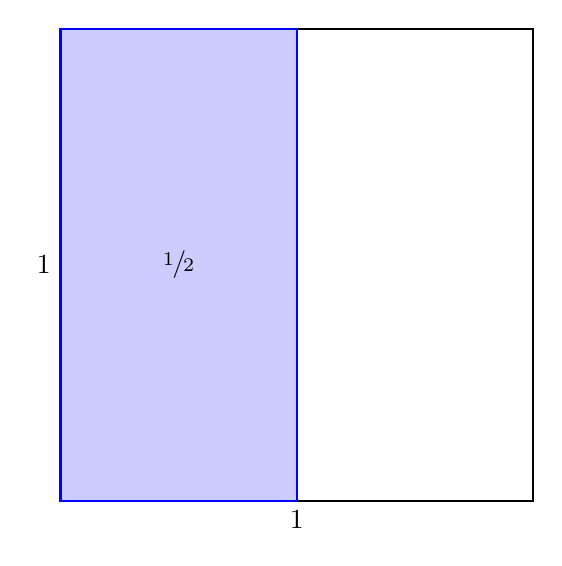
\begin{tikzpicture}[active/.style={thick, draw=blue, fill=blue!20}]
			\draw[thick] (0,0) rectangle (6,6);
			\node[left] at (0,3){1};
			\node[below] at (3,0){1};
			\draw[active] (0,0) rectangle (3,6) node[pos=.5] {$\sfrac{1}{2}$};
			\end{tikzpicture}
		\end{figure}
	\end{frame}

	\begin{frame}
		\begin{figure}
			\centering
			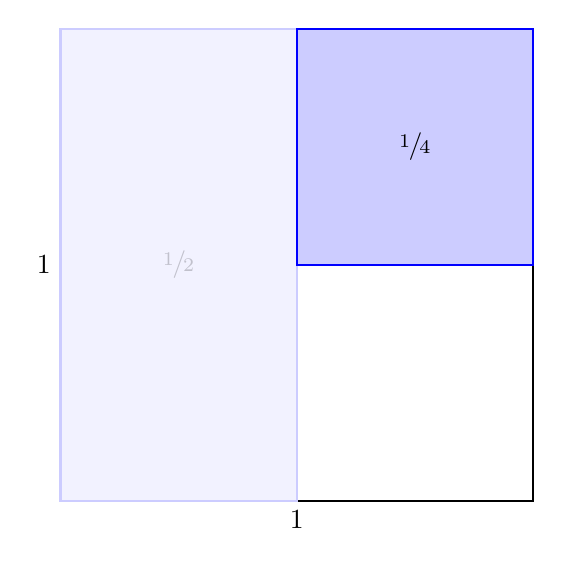
\begin{tikzpicture}[active/.style={thick, draw=blue, fill=blue!20}, inactive/.style={thick, draw=blue!20, fill=blue!5}]
			\draw[thick] (0,0) rectangle (6,6);
			\node[left] at (0,3){1};
			\node[below] at (3,0){1};
			\draw[inactive] (0,0) rectangle (3,6) node[pos=.5, opacity=.2] {$\sfrac{1}{2}$};
			\draw[active] (3,6) rectangle (6,3) node[pos=.5] {$\sfrac{1}{4}$};
			\end{tikzpicture}
		\end{figure}
	\end{frame}

	\begin{frame}
		\begin{figure}
			\centering
			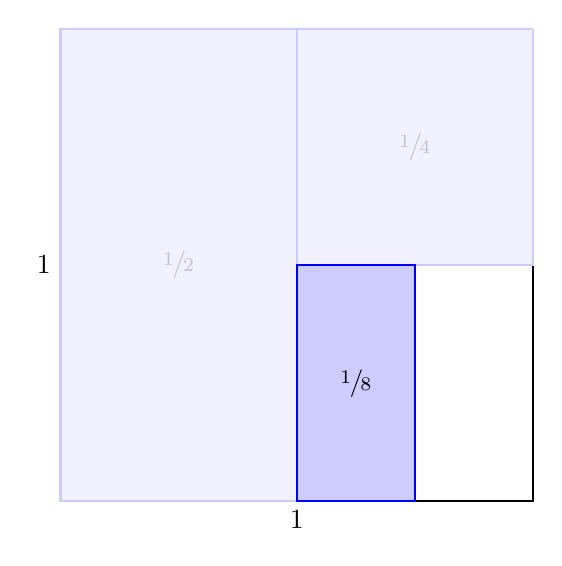
\begin{tikzpicture}[active/.style={thick, draw=blue, fill=blue!20}, inactive/.style={thick, draw=blue!20, fill=blue!5}]
			\draw[thick] (0,0) rectangle (6,6);
			\node[left] at (0,3){1};
			\node[below] at (3,0){1};
			\draw[inactive] (0,0) rectangle (3,6) node[pos=.5, opacity=.2] {$\sfrac{1}{2}$};
			\draw[inactive] (3,6) rectangle (6,3) node[pos=.5, opacity=.2] {$\sfrac{1}{4}$};
			\draw[active] (3,3) rectangle (4.5,0) node[pos=.5] {$\sfrac{1}{8}$};
			\end{tikzpicture}
		\end{figure}
	\end{frame}

	\begin{frame}
		\begin{figure}
			\centering
			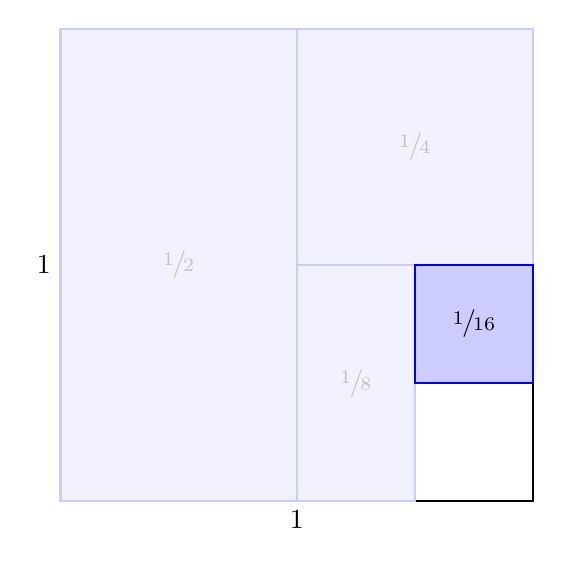
\begin{tikzpicture}[active/.style={thick, draw=blue, fill=blue!20}, inactive/.style={thick, draw=blue!20, fill=blue!5}]
			\draw[thick] (0,0) rectangle (6,6);
			\node[left] at (0,3){1};
			\node[below] at (3,0){1};
			\draw[inactive] (0,0) rectangle (3,6) node[pos=.5, opacity=.2] {$\sfrac{1}{2}$};
			\draw[inactive] (3,6) rectangle (6,3) node[pos=.5, opacity=.2]{$\sfrac{1}{4}$};
			\draw[inactive] (3,3) rectangle (4.5,0) node[pos=.5, opacity=.2] {$\sfrac{1}{8}$};
			\draw[active] (4.5,3) rectangle (6,1.5) node[pos=.5] {$\sfrac{1}{16}$};
			\end{tikzpicture}
		\end{figure}
	\end{frame}

	\begin{frame}
		\begin{figure}
			\centering
			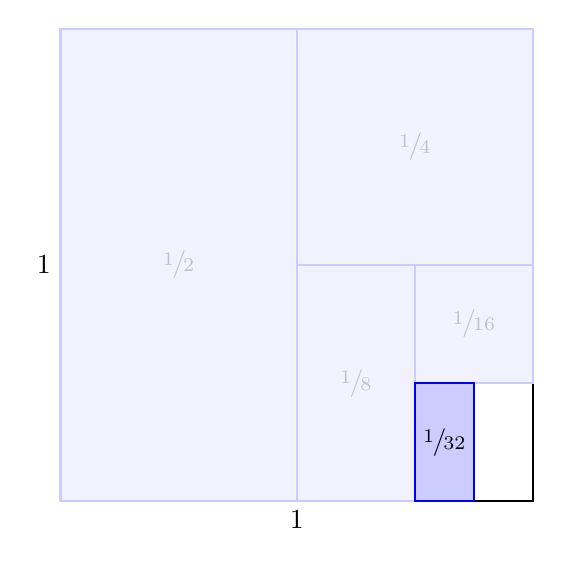
\begin{tikzpicture}[active/.style={thick, draw=blue, fill=blue!20}, inactive/.style={thick, draw=blue!20, fill=blue!5}]
			\draw[thick] (0,0) rectangle (6,6);
			\node[left] at (0,3){1};
			\node[below] at (3,0){1};
			\draw[inactive] (0,0) rectangle (3,6) node[pos=.5, opacity=.2] {$\sfrac{1}{2}$};
			\draw[inactive] (3,6) rectangle (6,3) node[pos=.5, opacity=.2]{$\sfrac{1}{4}$};
			\draw[inactive] (3,3) rectangle (4.5,0) node[pos=.5, opacity=.2] {$\sfrac{1}{8}$};
			\draw[inactive] (4.5,3) rectangle (6,1.5) node[pos=.5, opacity=.2] {$\sfrac{1}{16}$};
			\draw[active] (4.5,1.5) rectangle (5.25,0) node[pos=.5] {$\sfrac{1}{32}$};
			\end{tikzpicture}
		\end{figure}
	\end{frame}

	\begin{frame}
		\begin{figure}
			\centering
			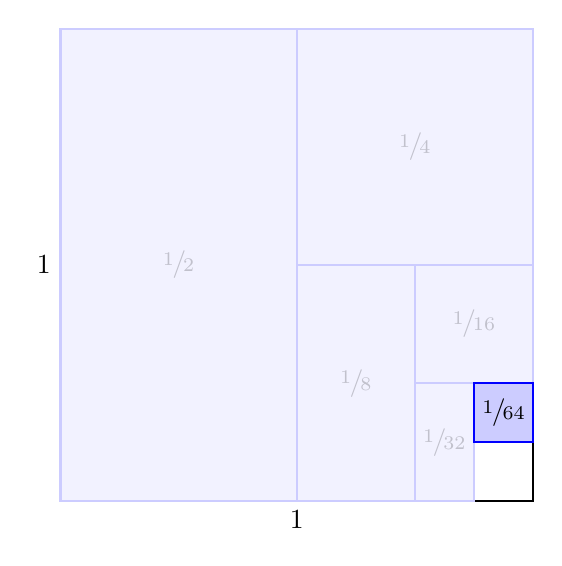
\begin{tikzpicture}[active/.style={thick, draw=blue, fill=blue!20}, inactive/.style={thick, draw=blue!20, fill=blue!5}]
			\draw[thick] (0,0) rectangle (6,6);
			\node[left] at (0,3){1};
			\node[below] at (3,0){1};
			\draw[inactive] (0,0) rectangle (3,6) node[pos=.5, opacity=.2] {$\sfrac{1}{2}$};
			\draw[inactive] (3,6) rectangle (6,3) node[pos=.5, opacity=.2]{$\sfrac{1}{4}$};
			\draw[inactive] (3,3) rectangle (4.5,0) node[pos=.5, opacity=.2] {$\sfrac{1}{8}$};
			\draw[inactive] (4.5,3) rectangle (6,1.5) node[pos=.5, opacity=.2] {$\sfrac{1}{16}$};
			\draw[inactive] (4.5,1.5) rectangle (5.25,0) node[pos=.5, opacity=.2] {$\sfrac{1}{32}$};
			\draw[active] (5.25,1.5) rectangle (6,.75) node[pos=.5] {$\sfrac{1}{64}$};
			\end{tikzpicture}
		\end{figure}
	\end{frame}

	\begin{frame}
		\begin{figure}
			\centering
			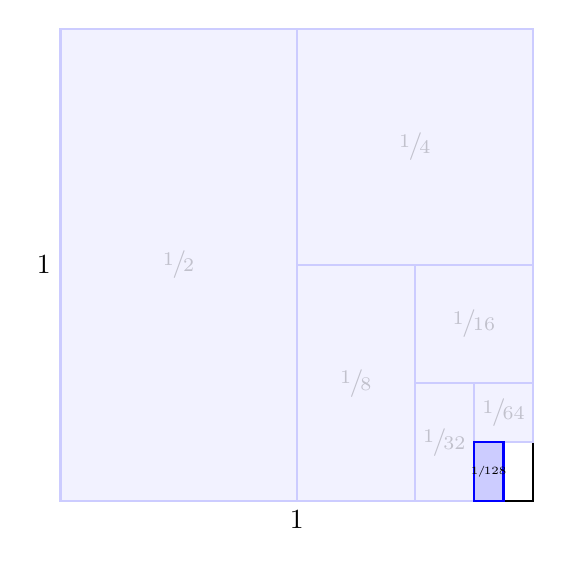
\begin{tikzpicture}[active/.style={thick, draw=blue, fill=blue!20}, inactive/.style={thick, draw=blue!20, fill=blue!5}]
			\draw[thick] (0,0) rectangle (6,6);
			\node[left] at (0,3){1};
			\node[below] at (3,0){1};
			\draw[inactive] (0,0) rectangle (3,6) node[pos=.5, opacity=.2] {$\sfrac{1}{2}$};
			\draw[inactive] (3,6) rectangle (6,3) node[pos=.5, opacity=.2]{$\sfrac{1}{4}$};
			\draw[inactive] (3,3) rectangle (4.5,0) node[pos=.5, opacity=.2] {$\sfrac{1}{8}$};
			\draw[inactive] (4.5,3) rectangle (6,1.5) node[pos=.5, opacity=.2] {$\sfrac{1}{16}$};
			\draw[inactive] (4.5,1.5) rectangle (5.25,0) node[pos=.5, opacity=.2] {$\sfrac{1}{32}$};
			\draw[inactive] (5.25,1.5) rectangle (6,.75) node[pos=.5, opacity=.2] {$\sfrac{1}{64}$};
			\draw[active] (5.25,.75) rectangle (5.625,0) node[pos=.5] {\scalebox{.8}{$\tiny\sfrac{1}{128}$}};
			\end{tikzpicture}
		\end{figure}
	\end{frame}
	
	\begin{frame}
		\begin{figure}
			\centering
			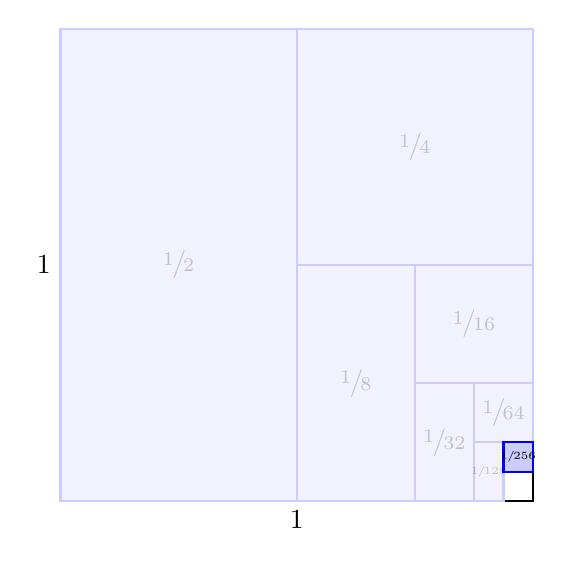
\begin{tikzpicture}[active/.style={thick, draw=blue, fill=blue!20}, inactive/.style={thick, draw=blue!20, fill=blue!5}]
			\draw[thick] (0,0) rectangle (6,6);
			\node[left] at (0,3){1};
			\node[below] at (3,0){1};
			\draw[inactive] (0,0) rectangle (3,6) node[pos=.5, opacity=.2] {$\sfrac{1}{2}$};
			\draw[inactive] (3,6) rectangle (6,3) node[pos=.5, opacity=.2]{$\sfrac{1}{4}$};
			\draw[inactive] (3,3) rectangle (4.5,0) node[pos=.5, opacity=.2] {$\sfrac{1}{8}$};
			\draw[inactive] (4.5,3) rectangle (6,1.5) node[pos=.5, opacity=.2] {$\sfrac{1}{16}$};
			\draw[inactive] (4.5,1.5) rectangle (5.25,0) node[pos=.5, opacity=.2] {$\sfrac{1}{32}$};
			\draw[inactive] (5.25,1.5) rectangle (6,.75) node[pos=.5, opacity=.2] {$\sfrac{1}{64}$};
			\draw[inactive] (5.25,.75) rectangle (5.625,0) node[pos=.5, opacity=.2] {\scalebox{.8}{$\tiny\sfrac{1}{128}$}};
			\draw[active] (5.625,.75) rectangle (6,.375) node[pos=.5] {\scalebox{.8}{$\tiny\sfrac{1}{256}$}};
			\end{tikzpicture}
		\end{figure}
	\end{frame}
\end{document}